\documentclass{article}
\usepackage[T1]{fontenc}
\usepackage[utf8]{vietnam}
\usepackage{amsmath}
\usepackage{graphicx}
\usepackage{color}
\usepackage{tikz}
\usepackage{indentfirst}
\usepackage[vietnamese,english]{babel}
\usepackage{fancyhdr}
\usepackage{lastpage}
\usepackage{csquotes}
\usepackage[colorinlistoftodos]{todonotes}
\usepackage[colorlinks=true, allcolors=blue]{hyperref}
\usepackage{wrapfig}
\usepackage{subfigure}
\usepackage[labelsep=endash]{caption}
\usepackage[figurename=Image]{caption}
% \renewcommand{\figurename}{Image}

\PassOptionsToPackage{hyphens}{url}\usepackage{hyperref}
\hypersetup{
	colorlinks=true,
	linkcolor=blue,
	filecolor=magenta,      
	urlcolor=cyan,
	pdftitle={Overleaf Example},
	pdfpagemode=FullScreen,
}

\graphicspath{{img/}}
\urlstyle{same}

\begin{document}
\begin{titlepage}
	\begin{center}
		\Huge
		\textbf{C++ Project Report}

		\vspace{0.5cm}
		\Large
		\textbf{The Horse Game}

		\vspace{10cm}
		\begin{minipage}{0.4\textwidth}
			\begin{flushleft} \large
				\emph{Student:}\\
				Phạm Xuân Việt Cường
			\end{flushleft}
		\end{minipage}
		~
		\begin{minipage}{0.4\textwidth}
			\begin{flushright} \large
				\emph{Teacher:} \\
				Hồ Thế Phúc
			\end{flushright}
		\end{minipage}\\[2cm]
	\end{center}
\end{titlepage}

\newpage
\tableofcontents

\newpage
\section{Introduction}
The Horse Game is inspired by a French board game called \emph{Jeu des petits chevaux}. We move some pawn (called horses) to the home reserved for their color. Each players received between 1 and 4 horses, the first players with all horses reach to home wins the game.

\begin{figure}[h]
	\centering
	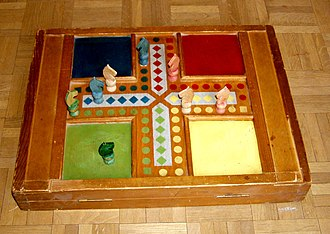
\includegraphics[width=0.5\textwidth]{small-horses}
	\label{fig:small-horses}
\end{figure}

\subsection{Rules}
Two or four players each have 1 to 4 pawns (horses). Play by rolling a dice in turn. PLayer must roll a 6 in order to remove a horse from start, that player need to make his horses move through all the square in the board.

\vspace{0.3cm}
\par
Player move a horse by roll dice, the number of dice that player rolled is the steps for the horse to move. If the horse moved to a square that already have another horse from other player, other player's horse will be send back to the start, if that another horse is the player's horse then the moving horse will stop just behind.

\vspace{0.3cm}
\par
After the horse has moved around the board, the horse need to go step-by-step to the center of the board by rolling the exact number of dice.

\vspace{0.3cm}
\par
The victory is won by the first player who manages to bring, according to variants, all of his horses to the cup.

\newpage

\section{Project}
\subsection{Basic}
The project Horse Game is a simple version of \emph{Jeu des petits chevaux}. The rules it still the same, but the board game is simplified. The board will now be a NxN size with two maps styles (image \ref{fig:map-style}). PLayer need to make all of his horses reach the end square to win.
\begin{figure}[h]
	\centering
	\subfigure[Spiral map]{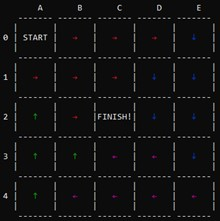
\includegraphics[width=0.45\textwidth]{spiral-map}}
	\subfigure[ZigZag map]{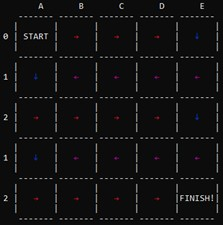
\includegraphics[width=0.45\textwidth]{zigzag-map}}

	\caption{Map Styles}
	\label{fig:map-style}
\end{figure}

\subsection{Code Explanation}
\subsubsection{Setup Game}
\begin{wrapfigure}{r}{0.55\textwidth}
	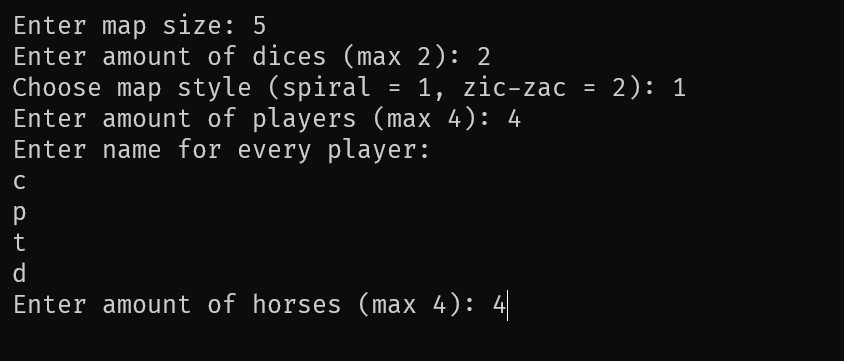
\includegraphics[width=0.55\textwidth]{setup}
	\caption{Setting up game}
	\label{fig:setup}
\end{wrapfigure}
When you start the game or replay it, first you need to setup game by entering some settings like in the image \ref{fig:setup}. After you finish setup the game, it'll show you the message: \textit{"Press any key to roll a dice"}. That mean you can play game now.

\subsubsection{Initializing board}
After you finish the game and prepare to play game, the program will Initializing the board with N size and maps style. For example, if you enter 5 for size and choose 1 (spiral map) the board will look like this:
\begin{figure}
	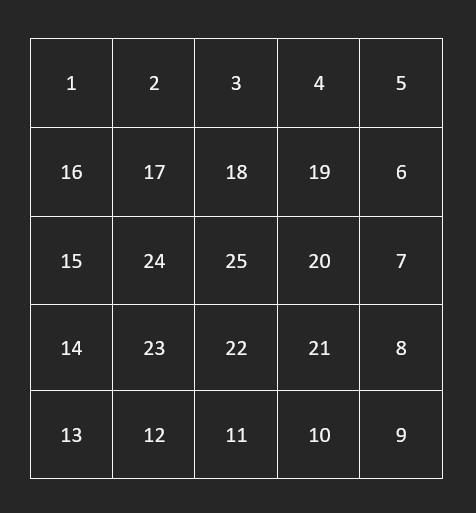
\includegraphics[width=1\textwidth]{example}
	\caption{Example}
	\label{fig:example}
\end{figure}
\end{document}